% interactcadsample.tex
% v1.03 - April 2017

\documentclass[]{interact}

\usepackage{epstopdf}% To incorporate .eps illustrations using PDFLaTeX, etc.
\usepackage{subfigure}% Support for small, `sub' figures and tables
%\usepackage[nolists,tablesfirst]{endfloat}% To `separate' figures and tables from text if required

\usepackage{natbib}% Citation support using natbib.sty
\bibpunct[, ]{(}{)}{;}{a}{}{,}% Citation support using natbib.sty
\renewcommand\bibfont{\fontsize{10}{12}\selectfont}% Bibliography support using natbib.sty

\theoremstyle{plain}% Theorem-like structures provided by amsthm.sty
\newtheorem{theorem}{Theorem}[section]
\newtheorem{lemma}[theorem]{Lemma}
\newtheorem{corollary}[theorem]{Corollary}
\newtheorem{proposition}[theorem]{Proposition}

\theoremstyle{definition}
\newtheorem{definition}[theorem]{Definition}
\newtheorem{example}[theorem]{Example}

\theoremstyle{remark}
\newtheorem{remark}{Remark}
\newtheorem{notation}{Notation}

% see https://stackoverflow.com/a/47122900

% Pandoc citation processing

\usepackage{hyperref}
\usepackage[utf8]{inputenc}
\def\tightlist{}
\usepackage{setspace}
\usepackage{graphicx}


\begin{document}

\articletype{Short Technical Note}

\title{A new simplified manual tour, with examples in mathematica and R}


\author{\name{Alex Aumann$^{a}$, German Valencia$^{a}$, Ursula
Laa$^{b}$, Dianne Cook$^{c}$}
\affil{$^{a}$School of Physics and Astronomy, Monash
University; $^{b}$Institute of Statistics, University of Natural
Resources and Life Sciences, Vienna; $^{b}$Department of Econometrics
and Business Statistics, Monash University}
}

\thanks{CONTACT Alex
Aumann. Email: \href{mailto:aaum0002@student.monash.edu}{\nolinkurl{aaum0002@student.monash.edu}}, German
Valencia. Email: \href{mailto:german.valencia@monash.edu}{\nolinkurl{german.valencia@monash.edu}}, Ursula
Laa. Email: \href{mailto:ursula.laa@boku.ac.at}{\nolinkurl{ursula.laa@boku.ac.at}}, Dianne
Cook. Email: \href{mailto:dicook@monash.edu}{\nolinkurl{dicook@monash.edu}}}

\maketitle

\begin{abstract}
Something here
\end{abstract}

\begin{keywords}
data visualisation; grand tour; statistical computing; statistical
graphics; multivariate data; dynamic graphics
\end{keywords}

\hypertarget{introduction}{%
\section{Introduction}\label{introduction}}

From a statistical perspective it is rare to have data that are strictly
3D, and so unlike in most computer graphics applications, the more
useful methods for data analysis show projections from an arbitrary
dimensional space. These are dynamic data visualizations methods and are
collected under the term \emph{tours}. Tours involve views of
high-dimensional (\(p\)) data in low-dimensional (\(d\)) projections. In
his original paper on the grand tour, \citet{As85} provided several
algorithms for tour paths that could theoretically show the viewer the
data \emph{from all sides}. Prior to Asimov's work, there were numerous
preparatory developments including \citet{tukey}'s PRIM-9. PRIM-9 had
user-controlled rotations on coordinate axes, allowing one to manually
tour through low-dimensional projections. It is impractical to
impossible to steer through all possible projections, unlike Asimov's
tours which allows one to quickly see many, many different projections.
After Asimov there have been many, many tour developments, as summarized
in \citet{lee2021}.

One such direction of work develops the ideas from PRIM-9, to provide
manual control of a tour. \citet{cook_manual_1997} describes controls
for 1D (or 2D) projections, in a 2D (or 3D) manipulation space, allowing
the user to select any variable axis, and rotate it into or out of or
around the projection through horizontal, vertical, oblique, radial or
angular changes in value. \citet{spyrison_spinifex_2020} refines this
algorithm and implements them to generate animations.

Manual controls are especially useful for assessing sensitivity of
structure to particular elements of the projection. There are many
places where it is useful. In exploratory data analysis, where one sees
clusters in a projection, can some variables be removed from the
projection without affecting the clustering. For interpreting models,
one can reduce or increase a variable's contribution to examine the
variable importance. These controls can also be used to interactively
generate facetted plots \citep{XXX}, or spatiotemporal glyphmaps
\citep{XXX}. Having the user interact with a projection is extremely
valuable for understanding high-dimensional data. However, these
algorithms have two problems: (1) the pre-processing of creating a
manipulation space overly complicates the algorithm, (2) extending to
higher dimensional control is difficult.

Through experiments with the relatively new interactive graphics
capabilities in mathematica(?), we have realized that there is a simpler
approach, which is more direct, and extensible for generating user
interaction. This paper explains this, and is organized as follows. The
next section describes the new algorithm for manual control. This is
followed by details on implementation. The applications section
illustrate how these can be used.

\hypertarget{sec:method}{%
\section{Manual tour}\label{sec:method}}

An orthonormal basis (\(A_{p\times d}\)) and a variable id
(\(m \in \{1, ..., p\}\)) to control are provided to initialise a manual
tour. A method to update the values of the component of the controlled
variable \(V_m\) is needed.

\hypertarget{background}{%
\subsection{Background}\label{background}}

In the original work, the method for updating component values, for a 2D
projection, was built trackball controls in 3D. A 3D manipulation space
is created, as illustrated in Figure \ref{manipspace}, where the
controlled variable has full range of motion from -1 to 1. Movements of
a cursor are recorded and converted into changes in the values of
\(V_m\) to change it's values in the displayed 2D projection. Movement
could also be constrained to be only in horizontal, vertical, radial or
angular motions.

\begin{figure*}[ht]
\centerline{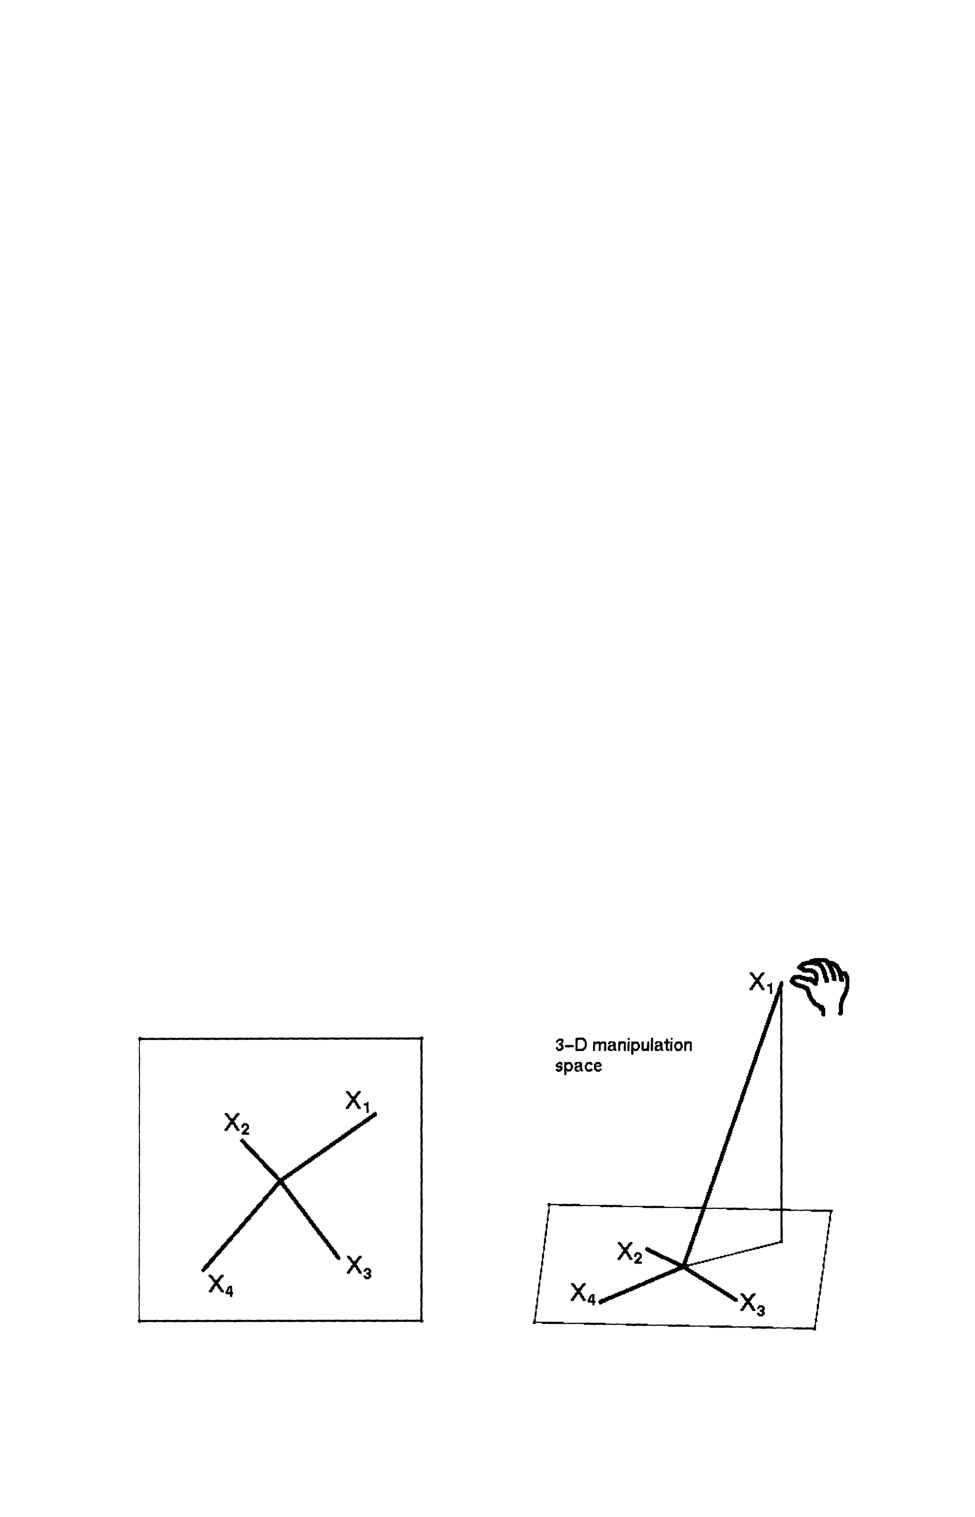
\includegraphics[width=0.8\textwidth]{figures/manip_space.pdf}}
\caption{Original contruction of the manual tour designed for 2D projections and created a 3D space from which to utilise track ball controls to change it's contribution. (Figure 3 from Cook and Buja (1997).)}
\label{manipspace}
\end{figure*}

\hypertarget{new-simpler-definition}{%
\subsection{New simpler definition}\label{new-simpler-definition}}

The new approach emerged from experiments in mathematica. The components
corresponding to \(V_m\) are directly controlled by cursor movement,
which updates row \(m\) of \(A\). The updated matrix is then
orthonormalised.

\hypertarget{algorithm-1}{%
\subsubsection{Algorithm 1}\label{algorithm-1}}

\begin{enumerate}
\def\labelenumi{\arabic{enumi}.}
\item
  Provide \(A\), and \(m\). (Note that \(m\) could also be automatically
  chosen as the component that is closest to the cursor position.)
\item
  Change values in row \(m\), giving \(A^*\). A large change in these
  values would correspond to making a large jump from the current
  projection. Small changes would correspond to tracking a cursor,
  making small jumps from the current projection.
\item
  Orthonormalise \(A^*\), using Gram-Schmidt. For \(d=2\), and
  \(A^* = \left[ {\boldmath a}_{.1}~{\boldmath a}_{.2}\right]\), the
  steps are:

  \begin{enumerate}
  \def\labelenumii{\roman{enumii}.}
  \tightlist
  \item
    Normalise \({\boldmath a}_{.1}\), and \({\boldmath a}_{.2}\).
  \item
    \({\boldmath a}^*_{.2} = {\boldmath a}_{.2} - {\boldmath a}_{.1}^T{\boldmath a}_{.2}{\boldmath a}_{.1}\).
  \item
    Normalise \({\boldmath a}^*_{.2}\).
  \end{enumerate}
\end{enumerate}

This algorithm will produce the changes to a projection as illustrated
in Figure \ref{fig:manualsequence} (top row). The controlled variable,
\(V_m\), corresponds to the black line, and sequential changes to row
\(m\) of \(A\) can be seen to roughly follow a specified position
(orange dot). Changes in the other components happen as a result of the
orthonormalisation, but are uncontrolled.

\hypertarget{algorithm-2}{%
\subsubsection{Algorithm 2}\label{algorithm-2}}

The problem with Algorithm 1 is that the precise values for \(V_m\)
cannot be specified because the orthonormalisation wil change them. This
modification will maintain the components of \(V_m\) precisely (Figure
\ref{fig:manualsequence} (bottom row)). The algorithm is as follows:

\begin{enumerate}
\def\labelenumi{\arabic{enumi}.}
\tightlist
\item
  Provide \(A\), and \(m\).
\item
  Change values in row \(m\), giving \(A^*\).
\item
  Store row \(m\) separately, and zero the values of row \(m\) in
  \(A^*\), giving \(A^{*0}\).
\item
  Orthonormalise \(A^{*0}\), using Gram-Schmidt.
\item
  Replace row \(m\) with the original values, giving \(A^{**}\).
\item
  For \(d=2\), adjust the values of \({\boldmath a}^{**}_{.2}\) using
\end{enumerate}

\[a^{**}_{j2}+\frac{a_{m1}a_{m2}}{p-1}, j=1, ..., p, j\neq m\].

which ensures that

\[\sum_{j=1, j\neq m}^p a^{**}_{j1}a^{**}_{j2} + a_{m1}a_{m2} = 0\].

If \(d>2\) the process would be sequentially repeated in the same manner
that Gram-Schmidt is applied sequentially to orthormalise the columns of
a matrix. If \(d=1\) no orthonormalisation is needed, and the projection
vector would simply need to be normalised after each adjustment.

\begin{figure}
\centering
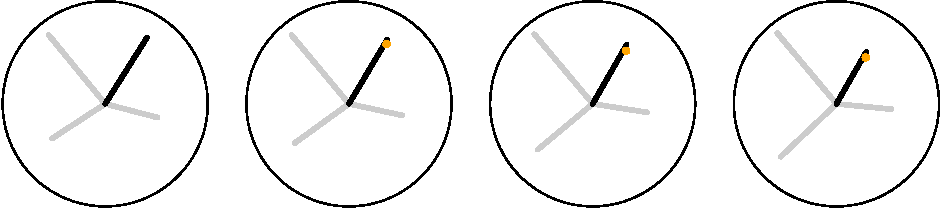
\includegraphics{paper_files/figure-latex/manualsequence-1.pdf}
\caption{Sequence of projections where contribution of one variable is
controlled (black) is changed: (top) unconstrained orthonormalisation,
(bottom) constrained as specified. The dot (orange) indicates the chosen
values for the controlled variable. For the constrained
orthonormalisation it can be seen to precisely match the axis, but not
so for the unconstrained orthonormalisation.}
\end{figure}

\hypertarget{potential-algorithm-3}{%
\subsubsection{Potential Algorithm 3}\label{potential-algorithm-3}}

For now just sketching the idea:

\begin{itemize}
\tightlist
\item
  first step is to click on the axis display to change the contribution
  of one variable \(m\)
\item
  capture that position and replace the corresponding row in the
  projection matrix
\item
  for 2D projection this gives components \(m_1\) along ``x'' direction
  and \(m_2\) along \(y\) direction
\item
  next step: rotate basis such that direction of row m now corresponds
  to the first basis vector, this means we apply 2x2 rotation matrix to
  each row of the projection matrix, where the rotation angle is
  \(tan(\theta) = m_2/m_1\) (that matrix can be written just in terms of
  that ratio, \(x= m_2/m_1\), when \(m_1<0\) I think we just need to
  translate \(\theta \rightarrow \theta + \pi\))
\item
  take the rotated basis, apply Gram-Schmidt, now the direction of \(m\)
  will not change (but the length will change during normalization)
\item
  rotated back to the original xy basis to update the plots
\end{itemize}

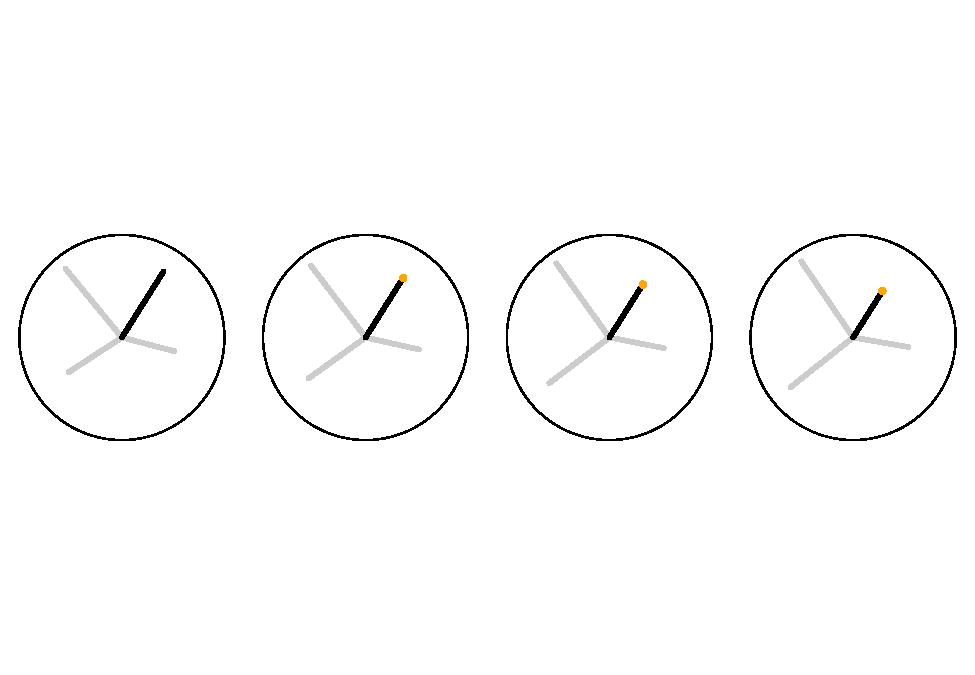
\includegraphics{paper_files/figure-latex/unnamed-chunk-1-1.pdf}

\hypertarget{sec:implementation}{%
\section{Implementation}\label{sec:implementation}}

\hypertarget{sec:examples}{%
\section{Applications}\label{sec:examples}}

\hypertarget{sec:discussion}{%
\section{Discussion}\label{sec:discussion}}

\hypertarget{acknowledgements}{%
\section*{Acknowledgements}\label{acknowledgements}}
\addcontentsline{toc}{section}{Acknowledgements}

The authors gratefully acknowledge the support of the Australian
Research Council. The paper was written in \texttt{rmarkdown}
\citep{rmarkdown} using \texttt{knitr} \citep{knitr}.

\hypertarget{supplementary-material}{%
\section*{Supplementary material}\label{supplementary-material}}
\addcontentsline{toc}{section}{Supplementary material}

The source material and animated gifs for this paper are available at

\bibliographystyle{tfcad}
\bibliography{biblio.bib}




\end{document}
